\section{Simulation Results}%
\label{sec:simulations}

In simulation section, we reverse the order by first showing the accuracy of estimators in carrier synchronization
and then showing some results of sequential detection since the GLRT sequential detector in~\eqref{eq:generalized_corr} relies on the accuracy of 
the single-lag estimator. The symbol sequence of the preamble is chosen as the Gold sequence and
modulated by a QPSK alphabet with good autocorrelation properties. The pulse is chosen
by $50\%$ rolloff Square-Root Raised Cosine (SRRC) pulse to satisfy the (squared root of) nyquist property.
The normalized frequency offset $\delta$ is intentionally set to be in the safe estimation range for all estimators for simulation purpose.

\subsection{Simulation Results for Estimation}

\begin{figure}[t]
    \centerline{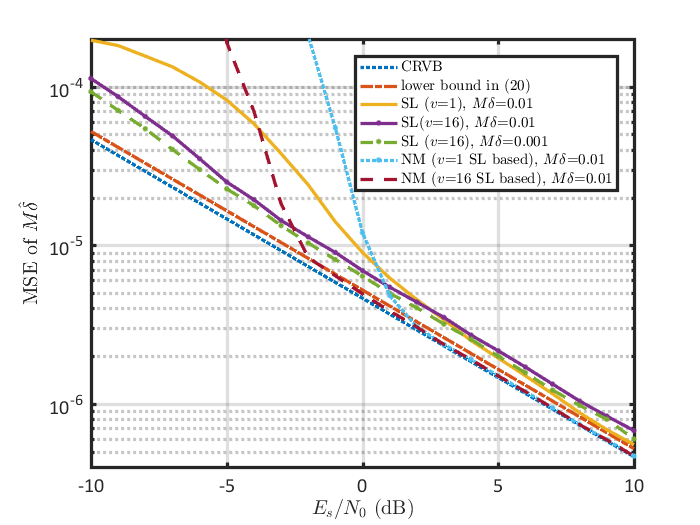
\includegraphics[width=3.05in]{accuracy_NM_SL.png}}
    \caption{Accuracy of the NM estimator and single-lag estimator ($L_0=32$)}
    \label{fig:accuracy_NM_SL}
    \end{figure}

\begin{figure}[t]
    \centerline{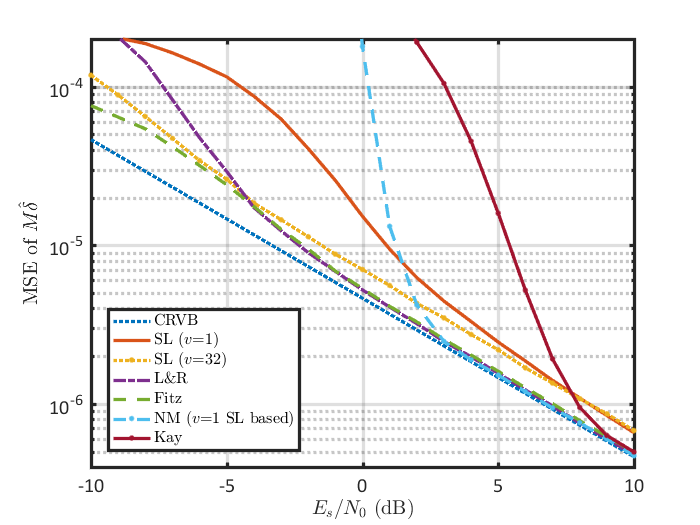
\includegraphics[width=3.05in]{accuracy_NM_SL_traditional.png}}
    \caption{Accuracy of SL, NM and traditional estimators ($L_0=32$, $M\delta=0.01$)}
    \label{fig:accuracy_NM_SL_traditional}
    \end{figure}

% \begin{figure}[t]
%     \centerline{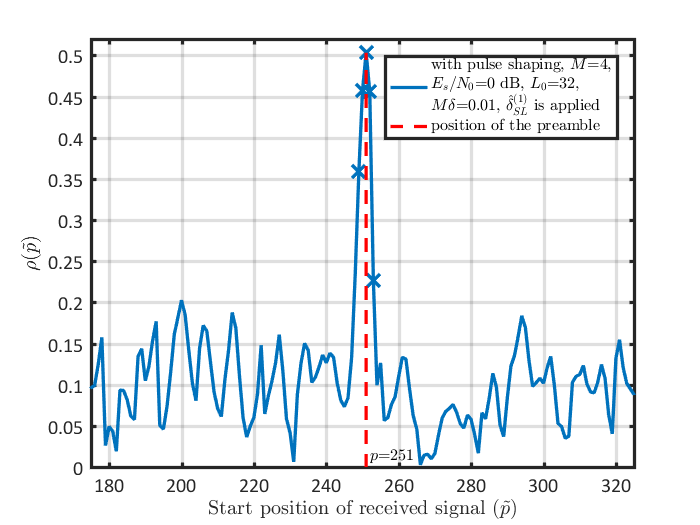
\includegraphics[width=3.4in]{generalized_correlation_p_plus_delta.png}}
%     \caption{Performance of sequential detector when the preamble is pulse shaped}
%     \label{fig:Generalized correlation}
%     \end{figure}

\begin{figure}[t]
    \centerline{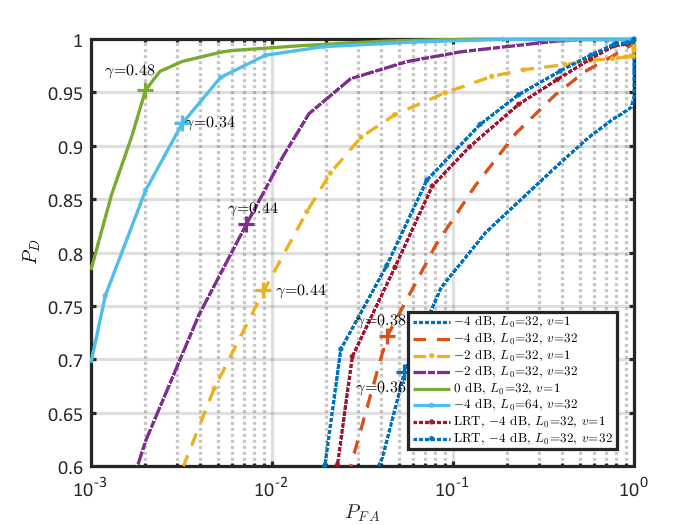
\includegraphics[width=3.05in]{ROC_new.png}}
    \caption{Receiver operating characteristics (ROC) of the sequential detector}
    \label{fig:Receiver operating characteristics}
    \end{figure}

Figure~\ref{fig:accuracy_NM_SL} illustrates the accuracy of single-lag (SL) and the NM estimator.
Compared with the two curves of SLs with $v{=}1$ and $v{=}16$, we see the length-$v$ partial correlating
improves the accuracy of SL by providing an approximate $2.5$ dB processing gain at negative SNRs.
Moreover, the SL with $v{=}1$ approaches the lower bound~\eqref{eq:lower_bound_single_lag_high_snr} at high SNRs
rather than SL with $v{=}16$. The gap is due to the Dirichlet function in~\eqref{eq:lower_bound_single_lag_high_snr} with respect to $v$ and $\delta$
increases the variance. For the same reason, the accuracy of SL with $v{=}16$ at small normalized frequency offset
has a better accuracy at all SNRs.

The SL estimators do not approach the CRVB~\cite{Gini_98} while the NM does. We also see the NM estimator gains 
a good accuracy based on the starting point of SL with $v{=}16$ at lower SNR due to the latter provides
an enough accuracy. In contrast, the NM estimator based on SL with $v{=}1$ has worse accuracy than SL 
at all negative SNRs because the accuracy of SL is not enough so that the Newton iteration converges occasionally to 
other local minimum away from the real frequency offset.

Figure~\ref{fig:accuracy_NM_SL_traditional} compares the accuracy of our proposed estimators
and the traditional estimators in~\cite{kay_89,Fitz_94,Luise_Reggiannini_95}. It shows at the small frequency offset environment,
our NM estimator even has a slightly better accuracy than traditional estimators at moderate SNRs.
The drawback of NM estimator is also obvious that the accuracy depends on the SL.
The figure also illustrates the lack of accuracy of single-lag estimators (our SL and Kay).

\subsection{Simulation Results for Detection}

% Figure~\ref{fig:Generalized correlation} shows the performance of sequential detector
% in~\eqref{eq:generalized_corr} at each received signal windows. Note, because of pulse sha-ping,
% the autocorrelation property of the preamble sequence is decreased, which results
% the correlations at adjacent windows near the position of the preamble decay slow and thus make much challenges
% to choose threshold to make correct dicision.

% The solution is to adjust the detection algorithm by finding the local maximum of the correlation
% instead of just comparing the correlation with the threshold at each window. Note, when count for the ratio of false alarm and detection (for determining the threshold),
% the two positions should be counted as latter.

Figure~\ref{fig:Receiver operating characteristics} shows the receiver operating characteristics (ROC) of the detection algorithm.
The better accuracy of SL with par-tial correlating at low SNRs also increases the performance of detection, e.g.,
at $-2$ dB SNR, $\gamma=0.56$, the gap of false alarm probability $P_{FA}$ is only $0.1\%$ but the detection probability $P_{D}$ of SL with $v{=}16$ is $5\%$ larger than $P_D$ of SL with $v{=}1$. 
The figure also shows the detector doesn't work well at $-4$ dB SNR if only $32$ symbols of preamble are used;  
The performance is significantly improved by doubling the number of symbols.
